%!TEX root = ../Main.tex

\chapter{implementation}

\section{Overview}
To give an overview of the software for the system, a class diagram has been made. This can be seen on \cref{fig:ClassDiagram}.
The class diagram have been developed based on the former domain problem analysis such as use cases. When a class diagram has been made that complies with the aforementioned use cases, it was used as a guideline for developing the system. Some changes have been made throughout the development when smarter options became apparent. \cref{fig:ClassDiagram} shows the latest class diagram for ROGSAnne.

\begin{figure}[H]
	\centering
	{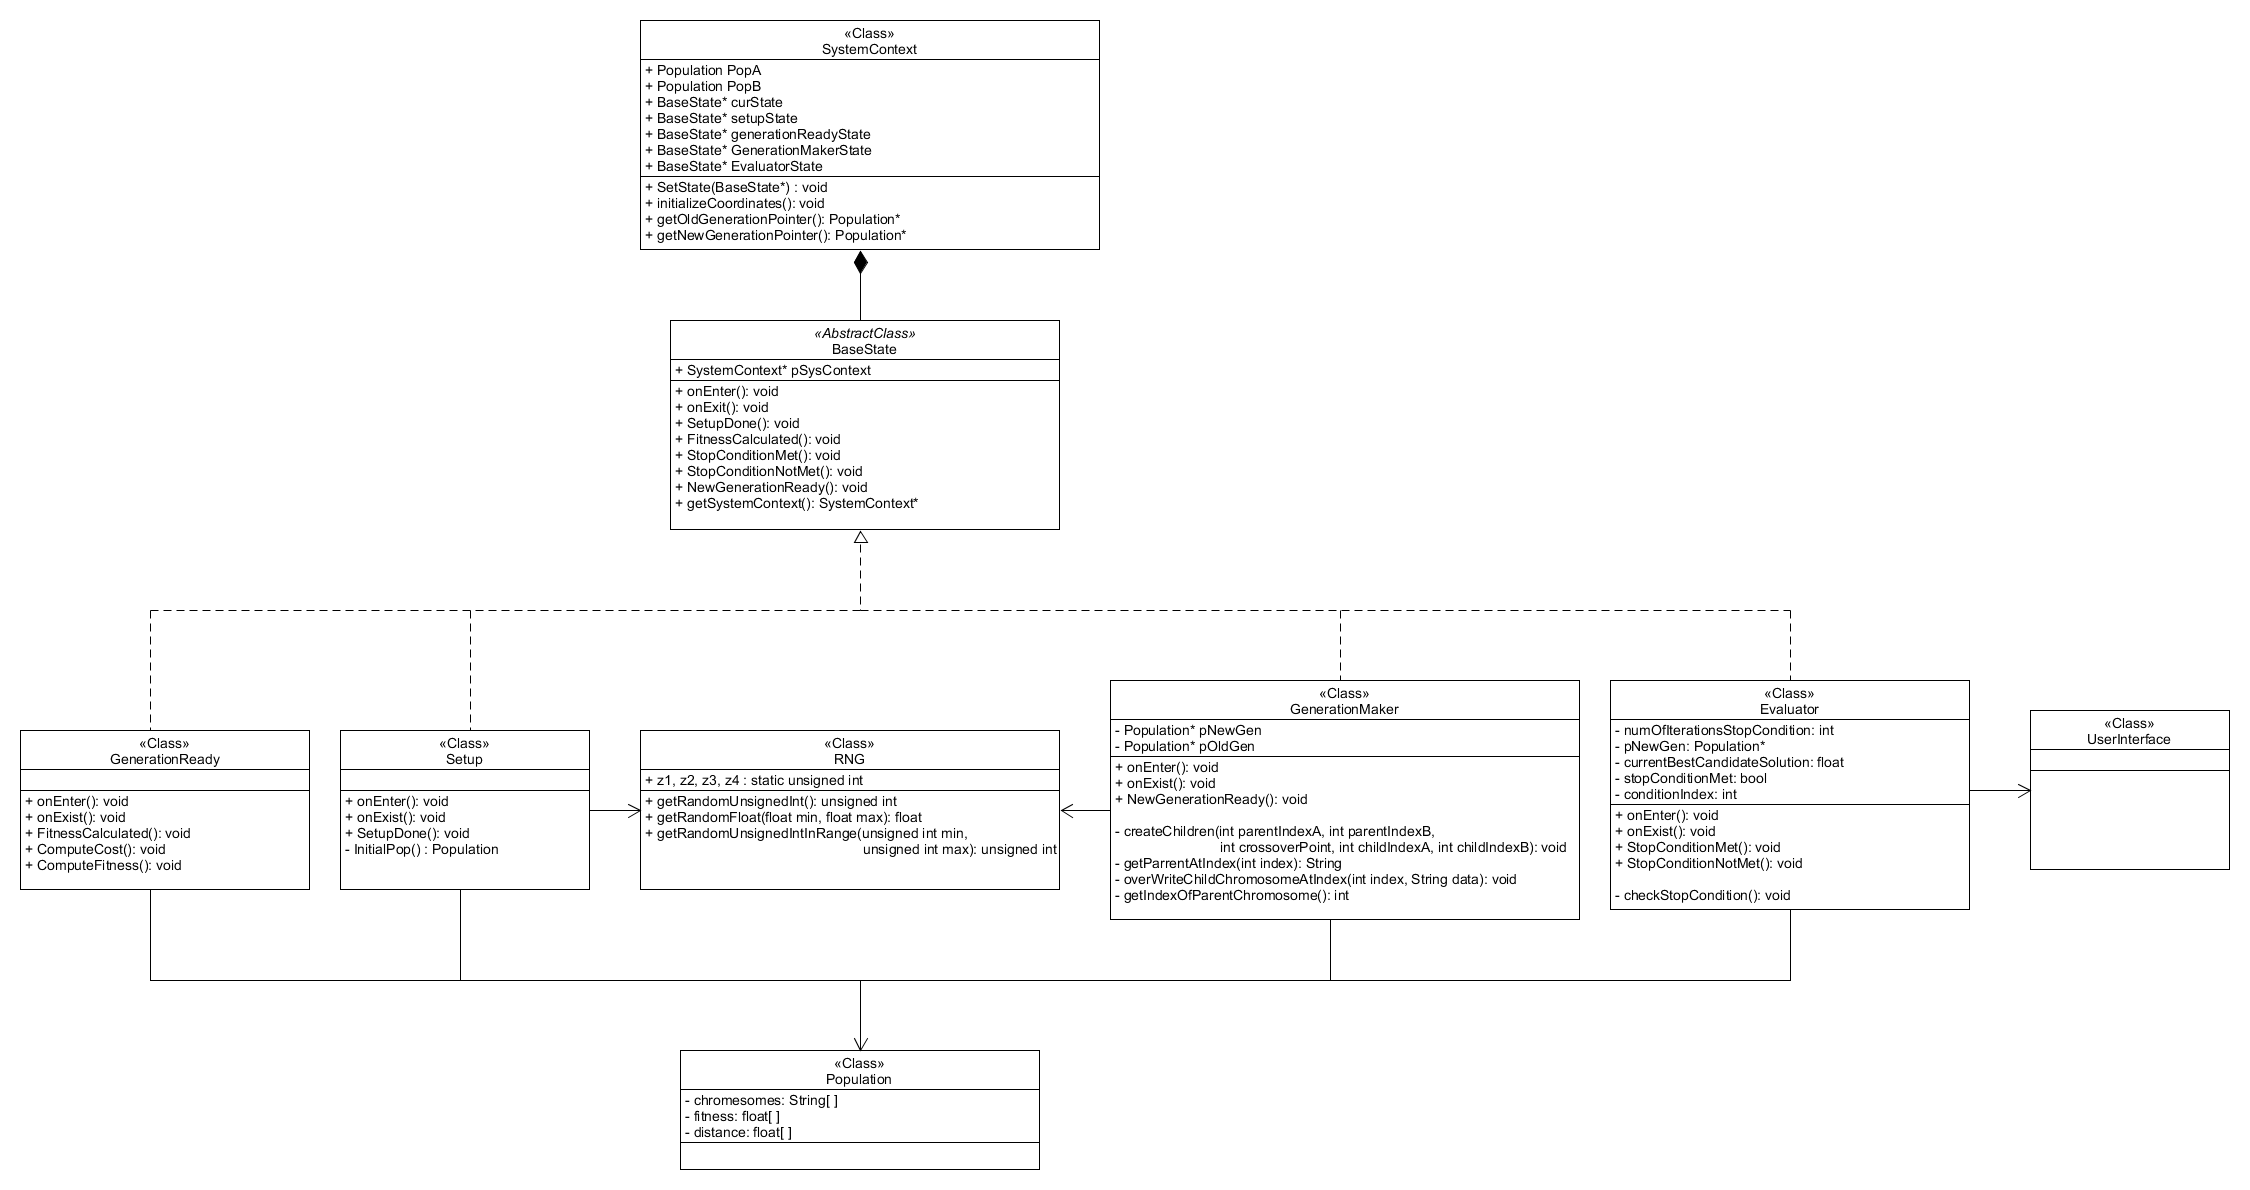
\includegraphics[width=\textwidth]{Images/ClassDiagram.PNG}}\\[0.5cm]
	\caption{Class diagram for the developed system.}
	\label{fig:ClassDiagram}
\end{figure}

As mentioned in the Design chapter a State Machine pattern has been chosen as a good fit for this system and a \textbf{SystemContext} class has been made to handle the holding and switching of states. The abstract class \textbf{Statebase} has virtual methods of each event needed for switching between states. Because StateBase is abstract each state class that inherits from the class needs to implement the corresponding method for changing state. I.e GenerationReady needs to implement FitnessCalculated() otherwise a default version will be called and an exception is called.

The four states functionality is described under the design chapter and can be summed up to:

\begin{itemize}
	\item \textbf{Setup}: Create initial population
	\item \textbf{GenerationReady}: Calculate distance and fitness of population
	\item \textbf{Evaluator}: Checks if there's been generated a better candidate solution, if not increment a counter. If this counter reaches a certain value, our stop condition is met and the program ends.
	\item \textbf{GenerationMaker}: Generate new population by taking the best of the population and use them as parents.
\end{itemize}



\section{SystemC}
